% Created by tikzDevice version 0.12
% !TEX encoding = UTF-8 Unicode
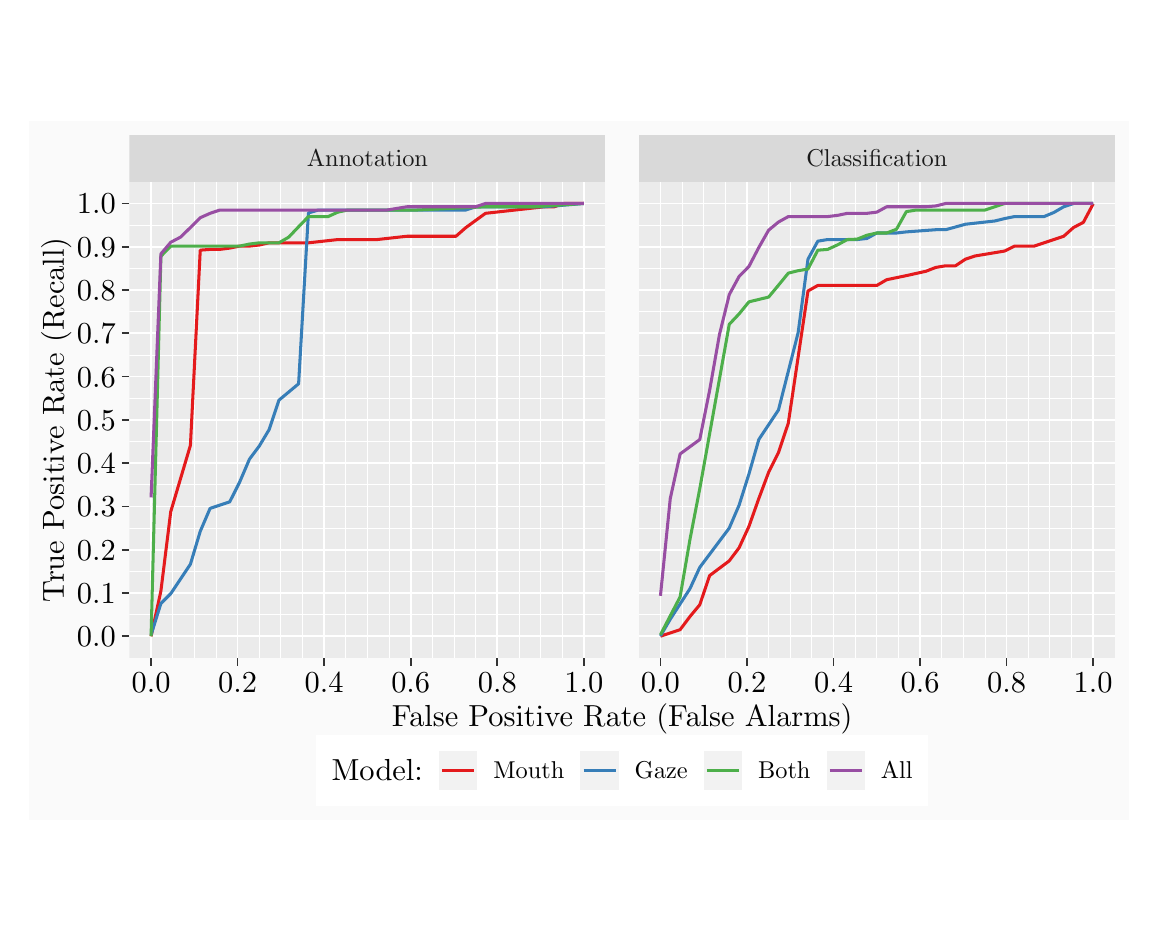
\begin{tikzpicture}[x=1pt,y=1pt]
\definecolor{fillColor}{RGB}{255,255,255}
\path[use as bounding box,fill=fillColor,fill opacity=0.00] (0,0) rectangle (398.34,320.03);
\begin{scope}
\path[clip] (  0.00, 33.41) rectangle (398.34,286.62);
\definecolor{drawColor}{RGB}{255,255,255}
\definecolor{fillColor}{gray}{0.98}

\path[draw=drawColor,line width= 0.6pt,line join=round,line cap=round,fill=fillColor] (  0.00, 33.41) rectangle (398.34,286.62);
\end{scope}
\begin{scope}
\path[clip] ( 36.77, 92.30) rectangle (208.78,264.31);
\definecolor{fillColor}{gray}{0.92}

\path[fill=fillColor] ( 36.77, 92.30) rectangle (208.78,264.31);
\definecolor{drawColor}{RGB}{255,255,255}

\path[draw=drawColor,line width= 0.3pt,line join=round] ( 36.77,107.94) --
	(208.78,107.94);

\path[draw=drawColor,line width= 0.3pt,line join=round] ( 36.77,123.58) --
	(208.78,123.58);

\path[draw=drawColor,line width= 0.3pt,line join=round] ( 36.77,139.22) --
	(208.78,139.22);

\path[draw=drawColor,line width= 0.3pt,line join=round] ( 36.77,154.85) --
	(208.78,154.85);

\path[draw=drawColor,line width= 0.3pt,line join=round] ( 36.77,170.49) --
	(208.78,170.49);

\path[draw=drawColor,line width= 0.3pt,line join=round] ( 36.77,186.13) --
	(208.78,186.13);

\path[draw=drawColor,line width= 0.3pt,line join=round] ( 36.77,201.77) --
	(208.78,201.77);

\path[draw=drawColor,line width= 0.3pt,line join=round] ( 36.77,217.40) --
	(208.78,217.40);

\path[draw=drawColor,line width= 0.3pt,line join=round] ( 36.77,233.04) --
	(208.78,233.04);

\path[draw=drawColor,line width= 0.3pt,line join=round] ( 36.77,248.68) --
	(208.78,248.68);

\path[draw=drawColor,line width= 0.3pt,line join=round] ( 52.41, 92.30) --
	( 52.41,264.31);

\path[draw=drawColor,line width= 0.3pt,line join=round] ( 60.23, 92.30) --
	( 60.23,264.31);

\path[draw=drawColor,line width= 0.3pt,line join=round] ( 68.05, 92.30) --
	( 68.05,264.31);

\path[draw=drawColor,line width= 0.3pt,line join=round] ( 83.68, 92.30) --
	( 83.68,264.31);

\path[draw=drawColor,line width= 0.3pt,line join=round] ( 91.50, 92.30) --
	( 91.50,264.31);

\path[draw=drawColor,line width= 0.3pt,line join=round] ( 99.32, 92.30) --
	( 99.32,264.31);

\path[draw=drawColor,line width= 0.3pt,line join=round] (114.96, 92.30) --
	(114.96,264.31);

\path[draw=drawColor,line width= 0.3pt,line join=round] (122.78, 92.30) --
	(122.78,264.31);

\path[draw=drawColor,line width= 0.3pt,line join=round] (130.60, 92.30) --
	(130.60,264.31);

\path[draw=drawColor,line width= 0.3pt,line join=round] (146.23, 92.30) --
	(146.23,264.31);

\path[draw=drawColor,line width= 0.3pt,line join=round] (154.05, 92.30) --
	(154.05,264.31);

\path[draw=drawColor,line width= 0.3pt,line join=round] (161.87, 92.30) --
	(161.87,264.31);

\path[draw=drawColor,line width= 0.3pt,line join=round] (177.51, 92.30) --
	(177.51,264.31);

\path[draw=drawColor,line width= 0.3pt,line join=round] (185.33, 92.30) --
	(185.33,264.31);

\path[draw=drawColor,line width= 0.3pt,line join=round] (193.15, 92.30) --
	(193.15,264.31);

\path[draw=drawColor,line width= 0.6pt,line join=round] ( 36.77,100.12) --
	(208.78,100.12);

\path[draw=drawColor,line width= 0.6pt,line join=round] ( 36.77,115.76) --
	(208.78,115.76);

\path[draw=drawColor,line width= 0.6pt,line join=round] ( 36.77,131.40) --
	(208.78,131.40);

\path[draw=drawColor,line width= 0.6pt,line join=round] ( 36.77,147.03) --
	(208.78,147.03);

\path[draw=drawColor,line width= 0.6pt,line join=round] ( 36.77,162.67) --
	(208.78,162.67);

\path[draw=drawColor,line width= 0.6pt,line join=round] ( 36.77,178.31) --
	(208.78,178.31);

\path[draw=drawColor,line width= 0.6pt,line join=round] ( 36.77,193.95) --
	(208.78,193.95);

\path[draw=drawColor,line width= 0.6pt,line join=round] ( 36.77,209.58) --
	(208.78,209.58);

\path[draw=drawColor,line width= 0.6pt,line join=round] ( 36.77,225.22) --
	(208.78,225.22);

\path[draw=drawColor,line width= 0.6pt,line join=round] ( 36.77,240.86) --
	(208.78,240.86);

\path[draw=drawColor,line width= 0.6pt,line join=round] ( 36.77,256.50) --
	(208.78,256.50);

\path[draw=drawColor,line width= 0.6pt,line join=round] ( 44.59, 92.30) --
	( 44.59,264.31);

\path[draw=drawColor,line width= 0.6pt,line join=round] ( 75.87, 92.30) --
	( 75.87,264.31);

\path[draw=drawColor,line width= 0.6pt,line join=round] (107.14, 92.30) --
	(107.14,264.31);

\path[draw=drawColor,line width= 0.6pt,line join=round] (138.41, 92.30) --
	(138.41,264.31);

\path[draw=drawColor,line width= 0.6pt,line join=round] (169.69, 92.30) --
	(169.69,264.31);

\path[draw=drawColor,line width= 0.6pt,line join=round] (200.96, 92.30) --
	(200.96,264.31);
\definecolor{drawColor}{RGB}{228,26,28}

\path[draw=drawColor,line width= 1.1pt,line join=round] ( 44.59,100.12) --
	( 48.14,116.47) --
	( 51.70,145.14) --
	( 58.81,169.13) --
	( 62.36,239.63) --
	( 65.91,239.91) --
	( 69.47,239.91) --
	( 73.02,240.38) --
	( 76.58,241.10) --
	( 80.13,241.10) --
	( 83.68,241.49) --
	( 87.24,242.28) --
	( 90.79,242.28) --
	( 94.35,242.28) --
	(101.45,242.28) --
	(112.12,243.47) --
	(115.67,243.47) --
	(119.22,243.47) --
	(122.78,243.47) --
	(126.33,243.47) --
	(136.99,244.65) --
	(140.55,244.65) --
	(144.10,244.65) --
	(147.66,244.65) --
	(151.21,244.65) --
	(154.76,244.65) --
	(158.32,247.78) --
	(165.42,252.94) --
	(176.09,254.13) --
	(186.75,255.31) --
	(190.30,255.31) --
	(193.86,256.50) --
	(197.41,256.50) --
	(200.96,256.50);
\definecolor{drawColor}{RGB}{55,126,184}

\path[draw=drawColor,line width= 1.1pt,line join=round] ( 44.59,100.62) --
	( 48.14,111.97) --
	( 51.70,115.52) --
	( 58.81,126.18) --
	( 62.36,138.03) --
	( 65.91,146.32) --
	( 73.02,148.69) --
	( 76.58,155.80) --
	( 80.13,164.09) --
	( 83.68,168.83) --
	( 87.24,174.76) --
	( 90.79,185.42) --
	( 97.90,191.34) --
	(101.45,253.07) --
	(105.01,254.13) --
	(108.56,254.13) --
	(115.67,254.13) --
	(119.22,254.13) --
	(126.33,254.13) --
	(133.44,254.13) --
	(140.55,254.13) --
	(144.10,254.13) --
	(147.66,254.13) --
	(154.76,254.13) --
	(158.32,254.13) --
	(161.87,255.31) --
	(165.42,255.31) --
	(172.53,255.31) --
	(179.64,255.31) --
	(186.75,255.31) --
	(193.86,255.90) --
	(200.96,256.50);
\definecolor{drawColor}{RGB}{77,175,74}

\path[draw=drawColor,line width= 1.1pt,line join=round] ( 44.59,100.12) --
	( 48.14,237.43) --
	( 51.70,241.10) --
	( 55.25,241.10) --
	( 58.81,241.10) --
	( 69.47,241.10) --
	( 73.02,241.10) --
	( 76.58,241.10) --
	( 80.13,241.84) --
	( 83.68,242.28) --
	( 87.24,242.28) --
	( 90.79,242.28) --
	( 94.35,244.35) --
	( 97.90,248.09) --
	(101.45,251.76) --
	(105.01,251.76) --
	(108.56,251.76) --
	(112.12,253.38) --
	(115.67,254.13) --
	(126.33,254.13) --
	(140.55,254.13) --
	(165.42,255.31) --
	(183.19,255.31) --
	(200.96,256.50);
\definecolor{drawColor}{RGB}{152,78,163}

\path[draw=drawColor,line width= 1.1pt,line join=round] ( 44.59,150.27) --
	( 48.14,238.29) --
	( 51.70,242.48) --
	( 55.25,244.35) --
	( 58.81,247.81) --
	( 62.36,251.36) --
	( 65.91,252.94) --
	( 69.47,254.13) --
	( 73.02,254.13) --
	( 76.58,254.13) --
	( 80.13,254.13) --
	( 83.68,254.13) --
	( 94.35,254.13) --
	( 97.90,254.13) --
	(101.45,254.13) --
	(105.01,254.13) --
	(108.56,254.13) --
	(119.22,254.13) --
	(122.78,254.13) --
	(129.89,254.13) --
	(136.99,255.31) --
	(147.66,255.31) --
	(161.87,255.31) --
	(165.42,256.50) --
	(168.98,256.50) --
	(200.96,256.50);
\end{scope}
\begin{scope}
\path[clip] (220.83, 92.30) rectangle (392.84,264.31);
\definecolor{fillColor}{gray}{0.92}

\path[fill=fillColor] (220.83, 92.30) rectangle (392.84,264.31);
\definecolor{drawColor}{RGB}{255,255,255}

\path[draw=drawColor,line width= 0.3pt,line join=round] (220.83,107.94) --
	(392.84,107.94);

\path[draw=drawColor,line width= 0.3pt,line join=round] (220.83,123.58) --
	(392.84,123.58);

\path[draw=drawColor,line width= 0.3pt,line join=round] (220.83,139.22) --
	(392.84,139.22);

\path[draw=drawColor,line width= 0.3pt,line join=round] (220.83,154.85) --
	(392.84,154.85);

\path[draw=drawColor,line width= 0.3pt,line join=round] (220.83,170.49) --
	(392.84,170.49);

\path[draw=drawColor,line width= 0.3pt,line join=round] (220.83,186.13) --
	(392.84,186.13);

\path[draw=drawColor,line width= 0.3pt,line join=round] (220.83,201.77) --
	(392.84,201.77);

\path[draw=drawColor,line width= 0.3pt,line join=round] (220.83,217.40) --
	(392.84,217.40);

\path[draw=drawColor,line width= 0.3pt,line join=round] (220.83,233.04) --
	(392.84,233.04);

\path[draw=drawColor,line width= 0.3pt,line join=round] (220.83,248.68) --
	(392.84,248.68);

\path[draw=drawColor,line width= 0.3pt,line join=round] (236.47, 92.30) --
	(236.47,264.31);

\path[draw=drawColor,line width= 0.3pt,line join=round] (244.28, 92.30) --
	(244.28,264.31);

\path[draw=drawColor,line width= 0.3pt,line join=round] (252.10, 92.30) --
	(252.10,264.31);

\path[draw=drawColor,line width= 0.3pt,line join=round] (267.74, 92.30) --
	(267.74,264.31);

\path[draw=drawColor,line width= 0.3pt,line join=round] (275.56, 92.30) --
	(275.56,264.31);

\path[draw=drawColor,line width= 0.3pt,line join=round] (283.38, 92.30) --
	(283.38,264.31);

\path[draw=drawColor,line width= 0.3pt,line join=round] (299.01, 92.30) --
	(299.01,264.31);

\path[draw=drawColor,line width= 0.3pt,line join=round] (306.83, 92.30) --
	(306.83,264.31);

\path[draw=drawColor,line width= 0.3pt,line join=round] (314.65, 92.30) --
	(314.65,264.31);

\path[draw=drawColor,line width= 0.3pt,line join=round] (330.29, 92.30) --
	(330.29,264.31);

\path[draw=drawColor,line width= 0.3pt,line join=round] (338.11, 92.30) --
	(338.11,264.31);

\path[draw=drawColor,line width= 0.3pt,line join=round] (345.93, 92.30) --
	(345.93,264.31);

\path[draw=drawColor,line width= 0.3pt,line join=round] (361.56, 92.30) --
	(361.56,264.31);

\path[draw=drawColor,line width= 0.3pt,line join=round] (369.38, 92.30) --
	(369.38,264.31);

\path[draw=drawColor,line width= 0.3pt,line join=round] (377.20, 92.30) --
	(377.20,264.31);

\path[draw=drawColor,line width= 0.6pt,line join=round] (220.83,100.12) --
	(392.84,100.12);

\path[draw=drawColor,line width= 0.6pt,line join=round] (220.83,115.76) --
	(392.84,115.76);

\path[draw=drawColor,line width= 0.6pt,line join=round] (220.83,131.40) --
	(392.84,131.40);

\path[draw=drawColor,line width= 0.6pt,line join=round] (220.83,147.03) --
	(392.84,147.03);

\path[draw=drawColor,line width= 0.6pt,line join=round] (220.83,162.67) --
	(392.84,162.67);

\path[draw=drawColor,line width= 0.6pt,line join=round] (220.83,178.31) --
	(392.84,178.31);

\path[draw=drawColor,line width= 0.6pt,line join=round] (220.83,193.95) --
	(392.84,193.95);

\path[draw=drawColor,line width= 0.6pt,line join=round] (220.83,209.58) --
	(392.84,209.58);

\path[draw=drawColor,line width= 0.6pt,line join=round] (220.83,225.22) --
	(392.84,225.22);

\path[draw=drawColor,line width= 0.6pt,line join=round] (220.83,240.86) --
	(392.84,240.86);

\path[draw=drawColor,line width= 0.6pt,line join=round] (220.83,256.50) --
	(392.84,256.50);

\path[draw=drawColor,line width= 0.6pt,line join=round] (228.65, 92.30) --
	(228.65,264.31);

\path[draw=drawColor,line width= 0.6pt,line join=round] (259.92, 92.30) --
	(259.92,264.31);

\path[draw=drawColor,line width= 0.6pt,line join=round] (291.20, 92.30) --
	(291.20,264.31);

\path[draw=drawColor,line width= 0.6pt,line join=round] (322.47, 92.30) --
	(322.47,264.31);

\path[draw=drawColor,line width= 0.6pt,line join=round] (353.75, 92.30) --
	(353.75,264.31);

\path[draw=drawColor,line width= 0.6pt,line join=round] (385.02, 92.30) --
	(385.02,264.31);
\definecolor{drawColor}{RGB}{228,26,28}

\path[draw=drawColor,line width= 1.1pt,line join=round] (228.65,100.15) --
	(232.20,101.31) --
	(235.75,102.49) --
	(239.31,107.23) --
	(242.86,111.50) --
	(246.42,122.04) --
	(253.52,127.37) --
	(257.08,132.11) --
	(260.63,139.81) --
	(264.19,149.88) --
	(267.74,159.36) --
	(271.29,166.46) --
	(274.85,177.12) --
	(281.96,224.88) --
	(285.51,226.88) --
	(289.06,226.88) --
	(292.62,226.88) --
	(296.17,226.88) --
	(303.28,226.88) --
	(306.83,226.88) --
	(310.39,228.95) --
	(317.50,230.43) --
	(324.60,232.01) --
	(328.16,233.40) --
	(331.71,233.99) --
	(335.26,233.99) --
	(338.82,236.36) --
	(342.37,237.54) --
	(349.48,238.73) --
	(353.03,239.32) --
	(356.59,241.10) --
	(360.14,241.10) --
	(363.70,241.10) --
	(367.25,242.28) --
	(370.80,243.47) --
	(374.36,244.65) --
	(377.91,247.81) --
	(381.47,249.68) --
	(385.02,256.38);
\definecolor{drawColor}{RGB}{55,126,184}

\path[draw=drawColor,line width= 1.1pt,line join=round] (228.65,100.22) --
	(232.20,106.28) --
	(239.31,117.30) --
	(242.86,125.00) --
	(246.42,129.74) --
	(253.52,139.22) --
	(257.08,147.51) --
	(260.63,158.76) --
	(264.19,171.20) --
	(271.29,181.86) --
	(278.40,209.79) --
	(281.96,236.36) --
	(285.51,242.87) --
	(289.06,243.47) --
	(292.62,243.47) --
	(299.73,243.47) --
	(303.28,243.86) --
	(306.83,245.83) --
	(313.94,245.83) --
	(317.50,246.23) --
	(328.16,247.02) --
	(331.71,247.02) --
	(338.82,248.99) --
	(349.48,250.18) --
	(353.03,251.05) --
	(356.59,251.76) --
	(360.14,251.76) --
	(367.25,251.76) --
	(370.80,253.24) --
	(374.36,255.31) --
	(377.91,256.50) --
	(381.47,256.50) --
	(385.02,256.50);
\definecolor{drawColor}{RGB}{77,175,74}

\path[draw=drawColor,line width= 1.1pt,line join=round] (228.65,100.66) --
	(235.75,114.34) --
	(239.31,135.07) --
	(242.86,153.43) --
	(253.52,212.84) --
	(257.08,216.61) --
	(260.63,220.96) --
	(267.74,222.68) --
	(271.29,226.96) --
	(274.85,231.32) --
	(278.40,232.21) --
	(281.96,232.80) --
	(285.51,239.61) --
	(289.06,239.91) --
	(292.62,241.53) --
	(296.17,243.47) --
	(299.73,243.61) --
	(303.28,245.04) --
	(306.83,245.83) --
	(310.39,245.83) --
	(313.94,247.19) --
	(317.50,253.55) --
	(321.05,254.13) --
	(324.60,254.13) --
	(328.16,254.13) --
	(331.71,254.13) --
	(338.82,254.13) --
	(342.37,254.13) --
	(345.93,254.13) --
	(349.48,255.31) --
	(353.03,256.50) --
	(356.59,256.50) --
	(360.14,256.50) --
	(363.70,256.50) --
	(370.80,256.50) --
	(374.36,256.50) --
	(377.91,256.50) --
	(381.47,256.50) --
	(385.02,256.50);
\definecolor{drawColor}{RGB}{152,78,163}

\path[draw=drawColor,line width= 1.1pt,line join=round] (228.65,114.73) --
	(232.20,149.88) --
	(235.75,165.99) --
	(242.86,171.20) --
	(246.42,188.97) --
	(249.97,209.11) --
	(253.52,223.58) --
	(257.08,230.14) --
	(260.63,233.76) --
	(264.19,240.59) --
	(267.74,246.85) --
	(271.29,249.79) --
	(274.85,251.76) --
	(278.40,251.76) --
	(281.96,251.76) --
	(285.51,251.76) --
	(289.06,251.76) --
	(292.62,252.20) --
	(296.17,252.94) --
	(303.28,252.94) --
	(306.83,253.37) --
	(310.39,255.31) --
	(313.94,255.31) --
	(317.50,255.31) --
	(321.05,255.31) --
	(324.60,255.31) --
	(328.16,255.61) --
	(331.71,256.50) --
	(335.26,256.50) --
	(338.82,256.50) --
	(345.93,256.50) --
	(353.03,256.50) --
	(356.59,256.50) --
	(360.14,256.50) --
	(367.25,256.50) --
	(377.91,256.50) --
	(385.02,256.50);
\end{scope}
\begin{scope}
\path[clip] ( 36.77,264.31) rectangle (208.78,281.12);
\definecolor{fillColor}{gray}{0.85}

\path[fill=fillColor] ( 36.77,264.31) rectangle (208.78,281.12);
\definecolor{drawColor}{gray}{0.10}

\node[text=drawColor,anchor=base,inner sep=0pt, outer sep=0pt, scale=  0.88] at (122.78,269.69) {Annotation};
\end{scope}
\begin{scope}
\path[clip] (220.83,264.31) rectangle (392.84,281.12);
\definecolor{fillColor}{gray}{0.85}

\path[fill=fillColor] (220.83,264.31) rectangle (392.84,281.12);
\definecolor{drawColor}{gray}{0.10}

\node[text=drawColor,anchor=base,inner sep=0pt, outer sep=0pt, scale=  0.88] at (306.83,269.69) {Classification};
\end{scope}
\begin{scope}
\path[clip] (  0.00,  0.00) rectangle (398.34,320.03);
\definecolor{drawColor}{gray}{0.20}

\path[draw=drawColor,line width= 0.6pt,line join=round] ( 44.59, 89.55) --
	( 44.59, 92.30);

\path[draw=drawColor,line width= 0.6pt,line join=round] ( 75.87, 89.55) --
	( 75.87, 92.30);

\path[draw=drawColor,line width= 0.6pt,line join=round] (107.14, 89.55) --
	(107.14, 92.30);

\path[draw=drawColor,line width= 0.6pt,line join=round] (138.41, 89.55) --
	(138.41, 92.30);

\path[draw=drawColor,line width= 0.6pt,line join=round] (169.69, 89.55) --
	(169.69, 92.30);

\path[draw=drawColor,line width= 0.6pt,line join=round] (200.96, 89.55) --
	(200.96, 92.30);
\end{scope}
\begin{scope}
\path[clip] (  0.00,  0.00) rectangle (398.34,320.03);
\definecolor{drawColor}{RGB}{0,0,0}

\node[text=drawColor,anchor=base,inner sep=0pt, outer sep=0pt, scale=  1.10] at ( 44.59, 79.78) {0.0};

\node[text=drawColor,anchor=base,inner sep=0pt, outer sep=0pt, scale=  1.10] at ( 75.87, 79.78) {0.2};

\node[text=drawColor,anchor=base,inner sep=0pt, outer sep=0pt, scale=  1.10] at (107.14, 79.78) {0.4};

\node[text=drawColor,anchor=base,inner sep=0pt, outer sep=0pt, scale=  1.10] at (138.41, 79.78) {0.6};

\node[text=drawColor,anchor=base,inner sep=0pt, outer sep=0pt, scale=  1.10] at (169.69, 79.78) {0.8};

\node[text=drawColor,anchor=base,inner sep=0pt, outer sep=0pt, scale=  1.10] at (200.96, 79.78) {1.0};
\end{scope}
\begin{scope}
\path[clip] (  0.00,  0.00) rectangle (398.34,320.03);
\definecolor{drawColor}{gray}{0.20}

\path[draw=drawColor,line width= 0.6pt,line join=round] (228.65, 89.55) --
	(228.65, 92.30);

\path[draw=drawColor,line width= 0.6pt,line join=round] (259.92, 89.55) --
	(259.92, 92.30);

\path[draw=drawColor,line width= 0.6pt,line join=round] (291.20, 89.55) --
	(291.20, 92.30);

\path[draw=drawColor,line width= 0.6pt,line join=round] (322.47, 89.55) --
	(322.47, 92.30);

\path[draw=drawColor,line width= 0.6pt,line join=round] (353.75, 89.55) --
	(353.75, 92.30);

\path[draw=drawColor,line width= 0.6pt,line join=round] (385.02, 89.55) --
	(385.02, 92.30);
\end{scope}
\begin{scope}
\path[clip] (  0.00,  0.00) rectangle (398.34,320.03);
\definecolor{drawColor}{RGB}{0,0,0}

\node[text=drawColor,anchor=base,inner sep=0pt, outer sep=0pt, scale=  1.10] at (228.65, 79.78) {0.0};

\node[text=drawColor,anchor=base,inner sep=0pt, outer sep=0pt, scale=  1.10] at (259.92, 79.78) {0.2};

\node[text=drawColor,anchor=base,inner sep=0pt, outer sep=0pt, scale=  1.10] at (291.20, 79.78) {0.4};

\node[text=drawColor,anchor=base,inner sep=0pt, outer sep=0pt, scale=  1.10] at (322.47, 79.78) {0.6};

\node[text=drawColor,anchor=base,inner sep=0pt, outer sep=0pt, scale=  1.10] at (353.75, 79.78) {0.8};

\node[text=drawColor,anchor=base,inner sep=0pt, outer sep=0pt, scale=  1.10] at (385.02, 79.78) {1.0};
\end{scope}
\begin{scope}
\path[clip] (  0.00,  0.00) rectangle (398.34,320.03);
\definecolor{drawColor}{RGB}{0,0,0}

\node[text=drawColor,anchor=base east,inner sep=0pt, outer sep=0pt, scale=  1.10] at ( 31.82, 96.33) {0.0};

\node[text=drawColor,anchor=base east,inner sep=0pt, outer sep=0pt, scale=  1.10] at ( 31.82,111.97) {0.1};

\node[text=drawColor,anchor=base east,inner sep=0pt, outer sep=0pt, scale=  1.10] at ( 31.82,127.61) {0.2};

\node[text=drawColor,anchor=base east,inner sep=0pt, outer sep=0pt, scale=  1.10] at ( 31.82,143.25) {0.3};

\node[text=drawColor,anchor=base east,inner sep=0pt, outer sep=0pt, scale=  1.10] at ( 31.82,158.88) {0.4};

\node[text=drawColor,anchor=base east,inner sep=0pt, outer sep=0pt, scale=  1.10] at ( 31.82,174.52) {0.5};

\node[text=drawColor,anchor=base east,inner sep=0pt, outer sep=0pt, scale=  1.10] at ( 31.82,190.16) {0.6};

\node[text=drawColor,anchor=base east,inner sep=0pt, outer sep=0pt, scale=  1.10] at ( 31.82,205.80) {0.7};

\node[text=drawColor,anchor=base east,inner sep=0pt, outer sep=0pt, scale=  1.10] at ( 31.82,221.43) {0.8};

\node[text=drawColor,anchor=base east,inner sep=0pt, outer sep=0pt, scale=  1.10] at ( 31.82,237.07) {0.9};

\node[text=drawColor,anchor=base east,inner sep=0pt, outer sep=0pt, scale=  1.10] at ( 31.82,252.71) {1.0};
\end{scope}
\begin{scope}
\path[clip] (  0.00,  0.00) rectangle (398.34,320.03);
\definecolor{drawColor}{gray}{0.20}

\path[draw=drawColor,line width= 0.6pt,line join=round] ( 34.02,100.12) --
	( 36.77,100.12);

\path[draw=drawColor,line width= 0.6pt,line join=round] ( 34.02,115.76) --
	( 36.77,115.76);

\path[draw=drawColor,line width= 0.6pt,line join=round] ( 34.02,131.40) --
	( 36.77,131.40);

\path[draw=drawColor,line width= 0.6pt,line join=round] ( 34.02,147.03) --
	( 36.77,147.03);

\path[draw=drawColor,line width= 0.6pt,line join=round] ( 34.02,162.67) --
	( 36.77,162.67);

\path[draw=drawColor,line width= 0.6pt,line join=round] ( 34.02,178.31) --
	( 36.77,178.31);

\path[draw=drawColor,line width= 0.6pt,line join=round] ( 34.02,193.95) --
	( 36.77,193.95);

\path[draw=drawColor,line width= 0.6pt,line join=round] ( 34.02,209.58) --
	( 36.77,209.58);

\path[draw=drawColor,line width= 0.6pt,line join=round] ( 34.02,225.22) --
	( 36.77,225.22);

\path[draw=drawColor,line width= 0.6pt,line join=round] ( 34.02,240.86) --
	( 36.77,240.86);

\path[draw=drawColor,line width= 0.6pt,line join=round] ( 34.02,256.50) --
	( 36.77,256.50);
\end{scope}
\begin{scope}
\path[clip] (  0.00,  0.00) rectangle (398.34,320.03);
\definecolor{drawColor}{RGB}{0,0,0}

\node[text=drawColor,anchor=base,inner sep=0pt, outer sep=0pt, scale=  1.10] at (214.81, 67.51) {False Positive Rate (False Alarms)};
\end{scope}
\begin{scope}
\path[clip] (  0.00,  0.00) rectangle (398.34,320.03);
\definecolor{drawColor}{RGB}{0,0,0}

\node[text=drawColor,rotate= 90.00,anchor=base,inner sep=0pt, outer sep=0pt, scale=  1.10] at ( 13.08,178.31) {True Positive Rate (Recall)};
\end{scope}
\begin{scope}
\path[clip] (  0.00,  0.00) rectangle (398.34,320.03);
\definecolor{fillColor}{RGB}{255,255,255}

\path[fill=fillColor] (104.30, 38.91) rectangle (325.31, 64.36);
\end{scope}
\begin{scope}
\path[clip] (  0.00,  0.00) rectangle (398.34,320.03);
\definecolor{drawColor}{RGB}{0,0,0}

\node[text=drawColor,anchor=base west,inner sep=0pt, outer sep=0pt, scale=  1.10] at (109.80, 47.84) {Model:};
\end{scope}
\begin{scope}
\path[clip] (  0.00,  0.00) rectangle (398.34,320.03);
\definecolor{drawColor}{RGB}{255,255,255}
\definecolor{fillColor}{gray}{0.95}

\path[draw=drawColor,line width= 0.6pt,line join=round,line cap=round,fill=fillColor] (148.29, 44.41) rectangle (162.74, 58.86);
\end{scope}
\begin{scope}
\path[clip] (  0.00,  0.00) rectangle (398.34,320.03);
\definecolor{drawColor}{RGB}{228,26,28}

\path[draw=drawColor,line width= 1.1pt,line join=round] (149.73, 51.63) -- (161.30, 51.63);
\end{scope}
\begin{scope}
\path[clip] (  0.00,  0.00) rectangle (398.34,320.03);
\definecolor{drawColor}{RGB}{255,255,255}
\definecolor{fillColor}{gray}{0.95}

\path[draw=drawColor,line width= 0.6pt,line join=round,line cap=round,fill=fillColor] (199.40, 44.41) rectangle (213.86, 58.86);
\end{scope}
\begin{scope}
\path[clip] (  0.00,  0.00) rectangle (398.34,320.03);
\definecolor{drawColor}{RGB}{55,126,184}

\path[draw=drawColor,line width= 1.1pt,line join=round] (200.85, 51.63) -- (212.41, 51.63);
\end{scope}
\begin{scope}
\path[clip] (  0.00,  0.00) rectangle (398.34,320.03);
\definecolor{drawColor}{RGB}{255,255,255}
\definecolor{fillColor}{gray}{0.95}

\path[draw=drawColor,line width= 0.6pt,line join=round,line cap=round,fill=fillColor] (243.98, 44.41) rectangle (258.43, 58.86);
\end{scope}
\begin{scope}
\path[clip] (  0.00,  0.00) rectangle (398.34,320.03);
\definecolor{drawColor}{RGB}{77,175,74}

\path[draw=drawColor,line width= 1.1pt,line join=round] (245.43, 51.63) -- (256.99, 51.63);
\end{scope}
\begin{scope}
\path[clip] (  0.00,  0.00) rectangle (398.34,320.03);
\definecolor{drawColor}{RGB}{255,255,255}
\definecolor{fillColor}{gray}{0.95}

\path[draw=drawColor,line width= 0.6pt,line join=round,line cap=round,fill=fillColor] (288.37, 44.41) rectangle (302.83, 58.86);
\end{scope}
\begin{scope}
\path[clip] (  0.00,  0.00) rectangle (398.34,320.03);
\definecolor{drawColor}{RGB}{152,78,163}

\path[draw=drawColor,line width= 1.1pt,line join=round] (289.82, 51.63) -- (301.38, 51.63);
\end{scope}
\begin{scope}
\path[clip] (  0.00,  0.00) rectangle (398.34,320.03);
\definecolor{drawColor}{RGB}{0,0,0}

\node[text=drawColor,anchor=base west,inner sep=0pt, outer sep=0pt, scale=  0.88] at (168.24, 48.60) {Mouth};
\end{scope}
\begin{scope}
\path[clip] (  0.00,  0.00) rectangle (398.34,320.03);
\definecolor{drawColor}{RGB}{0,0,0}

\node[text=drawColor,anchor=base west,inner sep=0pt, outer sep=0pt, scale=  0.88] at (219.36, 48.60) {Gaze};
\end{scope}
\begin{scope}
\path[clip] (  0.00,  0.00) rectangle (398.34,320.03);
\definecolor{drawColor}{RGB}{0,0,0}

\node[text=drawColor,anchor=base west,inner sep=0pt, outer sep=0pt, scale=  0.88] at (263.93, 48.60) {Both};
\end{scope}
\begin{scope}
\path[clip] (  0.00,  0.00) rectangle (398.34,320.03);
\definecolor{drawColor}{RGB}{0,0,0}

\node[text=drawColor,anchor=base west,inner sep=0pt, outer sep=0pt, scale=  0.88] at (308.33, 48.60) {All};
\end{scope}
\end{tikzpicture}
